% !TEX root=../../mt-motion-analysis.tex
%!TeX spellcheck = en-US
\chapter{Methods} \label{ch:method}
\section{Overview}
In this chapter the system for assessing POEs will be presented. This system is naturally divided into two parts where firstly the videos are analyzed. The first subsystem extracts body part coordinates of the subjects. This information is then passed to the second subsystem where it is used to calculate a score according to \cite{Nae2017}. The data used is presented in Section \ref{sec:met-data} and the two subsystems are described in Sections \ref{sec:met-loc} and \ref{sec:met-class} respectively.

\section{Data}\label{sec:met-data}
The data available is in the form of videos each containing one subject, recorded from the front. As discussed in Chapter \ref{ch:intro} the \gls{sls} task and the femoral valgus, pelvis, trunk, and KMFP \glspl{poe} is evaluated. Each video contains four-five repetitions and for each repetition the \glspl{poe} above have been scored according to Table \ref{tab:poes}. Along with the \gls{poe} scores a certainty score, describing the confidence of the physiotherapist assessing the videos, is provided. This is between 0 (certain) and 2 (uncertain) and when above 0 the uncertainty direction is provided as well. This certainty score is only available for the combined (median) score for all repetitions, i.e. one certainty score per video.

In total there are labeled videos from 103 different subjects and for some of the subjects there are videos of the task performed with both right and left leg. The number of labeled repetitions per video and \gls{poe} varies slightly. This variation is due to different factors such as all subjects not performing five repetitions, that the entire movement was not captured in the video (and thereby ignored by us), or that some specific \gls{poe} could not be evaluated from that specific video for some reason. The total amount of data for the different \glspl{poe} is summarized in Table \ref{tab:data}. From this data 22 of the repetition sequences (110 repetitions) where put aside as a test set. This corresponds to about 21\% of the available data. The test set was chosen from the set of unique subjects ensuring no data from the same subject is in both the training and test data.

The label distributions can be seen in Figure \ref{fig:label-dist} and it can be noted that for all \glspl{poe} there is a slight imbalance with fewer repetitions classified as Poor. The imbalance for \gls{kmfp} is very clear with about 80\% of the data classified as Good.

\begin{table}
 \centering
 \caption{Data available for the different POEs.}
 \label{tab:data}
 % \footnotesize
 % {\renewcommand{\arraystretch}{1.2}
 % {\tabulinesep=0.8mm
 \begin{tabu}[t]{cccc}
   \textbf{\gls{poe}} &
   \multicolumn{1}{c}{\begin{tabular}[c]{@{}c@{}}\textbf{Number of}\\\textbf{unique subjects}\end{tabular}} &
   \multicolumn{1}{c}{\begin{tabular}[c]{@{}c@{}}\textbf{Number of}\\\textbf{repetition sequences}\end{tabular}} &
   \multicolumn{1}{c}{\begin{tabular}[c]{@{}c@{}}\textbf{Number of}\\ \textbf{repetitions}\end{tabular}} \\ \hline \hline
   \textbf{Trunk} & 103 & 105 & 520 \\
   \textbf{Pelvis} & 103 & 105 & 519 \\
   \textbf{Femoral Valgus} & 103 & 107 & 530 \\
   \textbf{\gls{kmfp}} & 103 & 107 & 530

 \end{tabu}

\end{table}

\begin{figure}
  \centering
  \begin{subfigure}[t]{0.4\textwidth}
    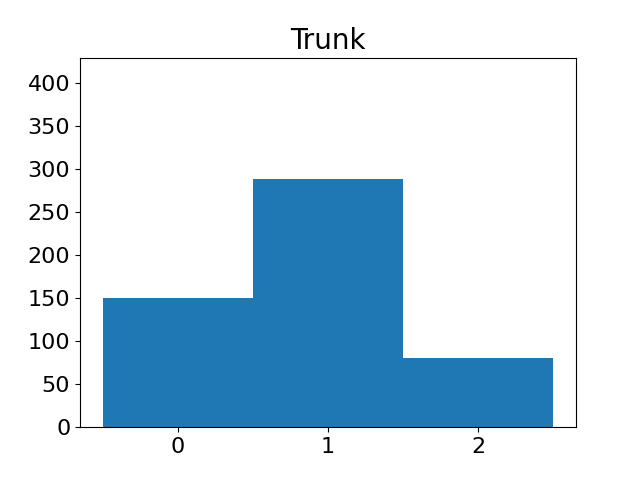
\includegraphics[width=\textwidth]{files/figs/met/trunk-label-hist.png}
    \caption{}
    \label{fig:trunk-labels}
  \end{subfigure}
  ~
  \begin{subfigure}[t]{0.4\textwidth}
    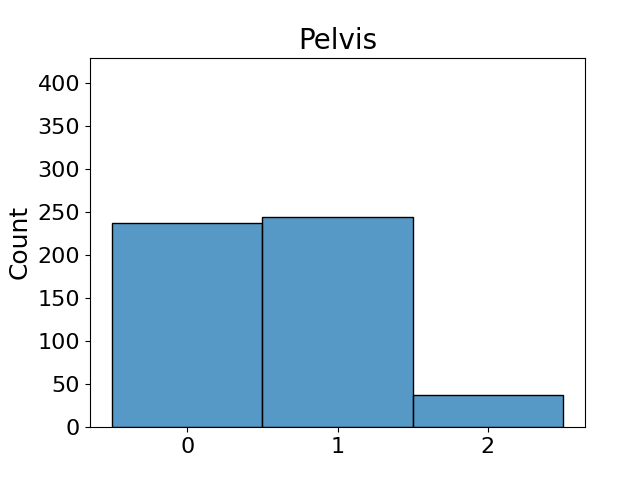
\includegraphics[width=\textwidth]{files/figs/met/pelvis-label-hist.png}
    \caption{}
    \label{fig:pelvis-labels}
  \end{subfigure}
  \begin{subfigure}[t]{0.4\textwidth}
    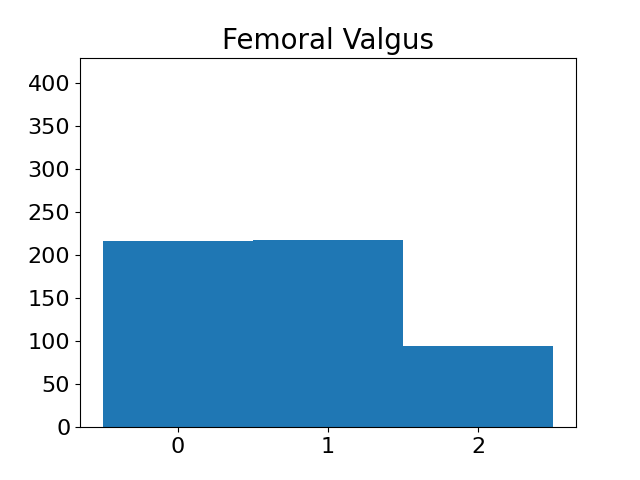
\includegraphics[width=\textwidth]{files/figs/met/femval-label-hist.png}
    \caption{}
    \label{fig:femval-labels}
  \end{subfigure}
  ~
  \begin{subfigure}[t]{0.4\textwidth}
    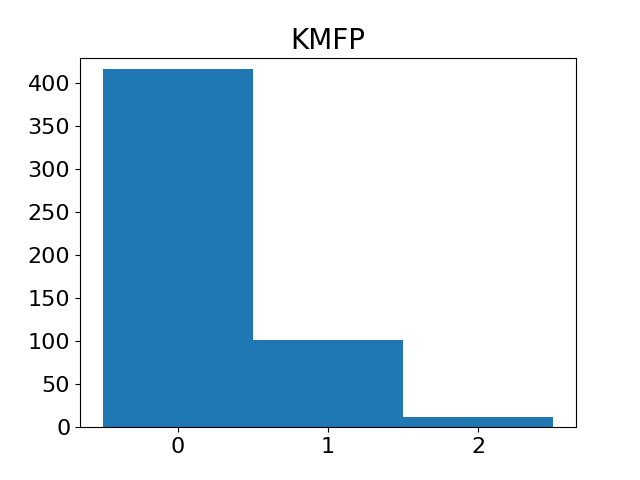
\includegraphics[width=\textwidth]{files/figs/met/kmfp-label-hist.png}
    \caption{}
    \label{fig:kmfp-labels}
  \end{subfigure}

  \caption{Distributions of the labels for the available data.}
  \label{fig:label-dist}
\end{figure}

 % performing four-five repetitions of specific motions. The motions are \textit{Single-leg squat, Forward lunge, Stair descending, Forward lunge, Single leg hop for distance, and Side hop}. Each motion has a number of POE scores associated with them. The motion-POE combinations are shown in Table \ref{tab:met:motion-poes}. In Sections \ref{sec:met-SLS}-\ref{} the motions and POEs evaluated in this project are described.

% The videos were recorded with different orientations and frame rates.
%
% The available videos has been assessed by a physiotherapist and for each repetition in each motion a number of POE scores has been awarded.


% \begin{table}
%  \centering
%  \caption{Motion-POE combinations available in the data.}
%  \label{tab:met:motion-poes}
%
%  \begin{tabular}{|c|ccccc|}
%   \hline
%   \backslashbox{POE}{Motion}                      &
%   \multicolumn{1}{c}{\begin{tabular}[c]{@{}c@{}}Single\\ leg squat\end{tabular}}   &
%   \multicolumn{1}{c}{\begin{tabular}[c]{@{}c@{}}Stair\\ descending\end{tabular}}   &
%   \multicolumn{1}{c}{\begin{tabular}[c]{@{}c@{}}Forward\\ lunge\end{tabular}}   &
%   \multicolumn{1}{c}{\begin{tabular}[c]{@{}c@{}}Single leg hop\\ for distance\end{tabular}}   &
%   \multicolumn{1}{c|}{\begin{tabular}[c]{@{}c@{}}Side\\ hop\end{tabular}}                      \\ \hline \hline
%
%   Trunk                                           & x & x &   & x & x \\ \hdashline
%   Hip                                             & x & x & x & x & x \\ \hdashline
%   \multicolumn{1}{|c|}{\begin{tabular}[c]{@{}c@{}}Femoral\\ valgus\end{tabular}} &
%   x                                               & x & x & x & x     \\ \hdashline
%   \multicolumn{1}{|c|}{\begin{tabular}[c]{@{}c@{}}Knee medial to\\ foot position\end{tabular}} &
%   x                                               & x & x & x & x     \\ \hdashline
%   \multicolumn{1}{|c|}{\begin{tabular}[c]{@{}c@{}}Femur medial\\ to shank\end{tabular}} &
%   x                                               & x & x & x & x     \\ \hdashline
%   Foot                                            & x &   &   &   &   \\ \hline
%  \end{tabular}
% \end{table}

% bara skriva om sls? om det bara 'r sls jag bed;mt.. ocks[ skriva det som avgr'nsningar

% \subsection{Single-leg squat, SLS} \label{sec:met-SLS}
% The subject performed a squat standing on one leg to a knee angle of approximately $60\degree$. The exercise was repeated five times and the entire movement was used to assess the POEs \cite{Nae2020}. An illustration is shown in Figure \ref{}.

% \subsection{Stair descending, SD}
% The subject stepped down from a 30 cm step board. The exercise was repeated five times and POEs were evaluated for the loaded leg during loading phase \cite{Nae2020}. An illustration is shown in Figure \ref{}.
%
% \subsection{Forward Lunge, FL}
%
% Helo I am now mispealing.



% The data the system is designed for is in the form of videos each containing around five repetitions of some specific motion. For each repetition in each motion up to five POEs has been graded according to \cite{Nae2017}.


\section{Body part localization} \label{sec:met-loc}
% \subsection{Preprocessing}
% ...
% rotation, flip etc
% \subsection{Pose estimation}
%The pose estimation can be seen as a feature extraction and dimensionality reduction.
The pose estimation is built around the open-source toolbox MMPose \cite{mmpose} from MMLab. Each frame is considered to be an independent image and is analyzed with a \gls{hrnet} model with the \gls{dark} extension trained on the \gls{coco}-wholebody dataset\footnote{The model used can be found here: \url{https://mmpose.readthedocs.io/en/latest/top_down_models.html}.}. Both the model and the dataset is described in Section \ref{sec:pose_estimation}. The extended wholebody dataset is used since it, along with the ankle positions, also estimates the positions of the toes and heels which according to Table \ref{tab:poes} ought to be important. % \ref{sec:hrnet, sec:dark, sec:coco}.

To get comparable results some of the videos were rotated and flipped before inferring the keypoints. This was needed since the videos were recorded in different orientations and the actions were performed with different legs. The rotations were based on the orientation of the subject (position of head w.r.t. the feet) in the first frame to have it standing up in the $y$-direction. Videos where the squats were performed with the left leg were then flipped around the $y$-axis to be able to use the same model for the left and right leg in a more efficient manner.

A bounding box for the subject is found using a Faster R-CNN model trained on the \gls{coco} dataset\footnote{The model used can be found here: \url{https://github.com/open-mmlab/mmdetection/tree/master/configs/faster_rcnn}.}. The content of this bounding box is resized to match the input size of the \gls{hpe} model used, 384$\times$288 pixels in our case. Each video analyzed results in sequences of $x$- and $y$-coordinates for all the keypoints in the dataset used to train the model.

%The file names contained information about which. The rotations were performed based on the position of the head with respect to the feet in the first frame.
\section{Classification} \label{sec:met-class}

\subsection{Preprocessing and dataset blabla..} \label{sec:met-class-preproc}
Before assessing the \glspl{poe} based on the body part positions a number of preprocessing steps are conducted. Firstly the data is resampled as the videos are recorded with a number of different frame rates ranging from 25 to 60 Hz. The resampling is performed using linear interpolation to a new sample frequency of 25Hz. This data is then low pass filtered through a fourth order Butterworth filter with a cutoff frequency of 2.5Hz. %PLOT P[ ;VERF;RING F;R FILTER? ELLER P[ FILTRERAD DATA?

While the \gls{poe} assessment is performed on a per repetition basis the body part coordinates are extracted on a per video or repetition sequence basis. Hence, the sequences corresponding to the entire video is split up in the individual repetitions. This splitting algorithm is presented in Algorithm \ref{alg:rep} and is based on finding the edges of the peaks in specific position data. For the \gls{sls} task the $y$-coordinate of the right shoulder is used. The number of points extracted for each repetition depends on the width of the peak. The length of the observed repetitions varies from about 1 to 8 seconds. For practical reasons, such as handling of data and training performance\footnote{All data in one batch must have the same size. Hence, to be able to train with a batch size larger than 1, which usually improves training performance \cite{Goodfellow2016}, all data in the same batch needs to have the same dimensions.}, it is desirable to save the data as multidimensional arrays with the same dimensions. Two different ways of solving this problem is evaluated, namely i) padding the sequences and use maskings for the padded samples in the models, and ii) alternate the sample frequency to thereby achieve sequences of the same length.
%Some number of points around each peak is  This is done by finding peaks in the sequences corresponding to certain body part positions. Which body part is used for this sequence splitting depends on which movement is analyzed.

\begin{algorithm}
\SetAlgoLined
% \KwResult{Write here the result }
%  initialization\;
% peaks, right\_edges, left\_edges = \textbf{find\_peaks}(sequence)\;
right\_edges, left\_edges = \textbf{find\_edges}(sequence)\;
 \For{\textup{peak, right, current\_left, next\_left} in \textup{peaks, right\_edges, left\_edges}}{
 % \For{\textup{peak, right, current\_left, next\_left} in \textup{peaks, right\_edges, left\_edges}}{
  split\_index = \textbf{mean}(right, next\_left)\;
  start = \textbf{max}(current\_left - extra\_points, 0)\;
  end = \textbf{min}(right + extra\_points, split\_index)\;
  % start = \textbf{max}(peak - max\_length/2, 0)\;
  % end = \textbf{min}(peak + max\_length/2, split\_index)\;
  \textit{repetition} = \textbf{normalize\_length}(sequence[start:end])\;
  sequence = sequence[end:]\;
 }
 \caption{Extraction of repetitions from sequences}
 \label{alg:rep}
\end{algorithm}


Finally the data is normalized. All coordinates are moved to put the mean position of the first five right hip-samples in the origin and are scaled to set the distance between the right shoulder and right hip to one, according to \eqref{eq:met-normalization}.

\begin{align}
  \begin{split}
    (x,y)_i &= (x,y)_i - {\mean{(x,y)}}_{rh} \\
    (x,y)_i &= \frac{(x,y)_i}{\lVert \mean{(x,y)}_{rs} \rVert_2} \qquad , \forall i
  \end{split}
  \label{eq:met-normalization}
\end{align}
\begin{conditions}
    $\mean{(x,y)}_i$  & =   & mean over first five samples for body part $i$ \\
    \textit{rh}     & =   & right hip \\
    \textit{rs}     & =   & right shoulder \\
    \textit{i}      & \in & Available body parts %\{body parts\}
\end{conditions}

After these preprocessing steps a dataset with inputs $\in \mathbb{R}^{N \times T \times F}$ and corresponding one-hot labels $\in \mathbb{Z}_3^N$ are created. The inputs consists of $N$ multivariate time series of length $T$ with $F$ channels. These channels are a subset of the extracted $x$- and $y$-coordinates as well as angles and differences between keypoints.

\subsection{Classifiers}
For the modeling we used ensembles of different deep learning based model architectures. The reasoning behind this was based on the results of Fawaz et al. \cite{IsmailFawaz2019ensemble}, suggesting that the output a deep learning model trained on a limited amount of data will vary based on the initial parameter values. By averaging the result over several models this variance will be reduced. Another reason for using an ensemble is, as can be seen in e.g. \cite{Bagnall2015, Lines2016}, that the combined result of many specialized models can be better than that of one more general model. %In this work it for instance mean that we can train models with the confusion-entropy loss \eqref{eq:confusion-entropy} to achieve e.g. high precision for just one class in combination with models trained with the \gls{coral} loss \eqref{eq:coral-loss} performing fairly good over all classes.

All models used have been modified to handle the padded input data discussed in Section \ref{sec:met-class-preproc}. This is done by adding masking layers setting the padded samples to zero throughout the networks, illustrated in Figure \ref{fig:x-inception}. This reduces the impact of the padded samples to something similar to the padding performed in convolutional layers to keep the size of the feature map intact. The same mask indicates which time steps should be ignored in the \gls{gap} layer.

The models eventually used were InceptionTime (Section \ref{sec:inception-time}) with different loss functions as well as an architecture designed by us, inspired by
\gls{xcm} (Section \ref{sec:XCM}) and InceptionTime. We call this model X-InceptionTime and it is presented below.

\textbf{skriv om ensemble, vilka losses}

\subsubsection{X-InceptionTime}
The idea with this model was to combine the explainability of XCM with the inception module from InceptionTime. This was done by separating the inputs and having individual inception modules for each input channel as can be seen in Figure \ref{fig:x-inception}. After the final module (the depth can be seen as a hyperparamtere and needs to be tuned) a bottleneck of size one is applied reducing the dimensionality of each input channel back to $T$$\times$1. The features for the individual inputs are concatenated resulting in a feature map of size $T$$\times$$F$ where each input feature is only affected by that input. This makes it possible to use \gls{grad-cam} to get a measure of the importance of each time step for each input.

\begin{figure}
  \centering
  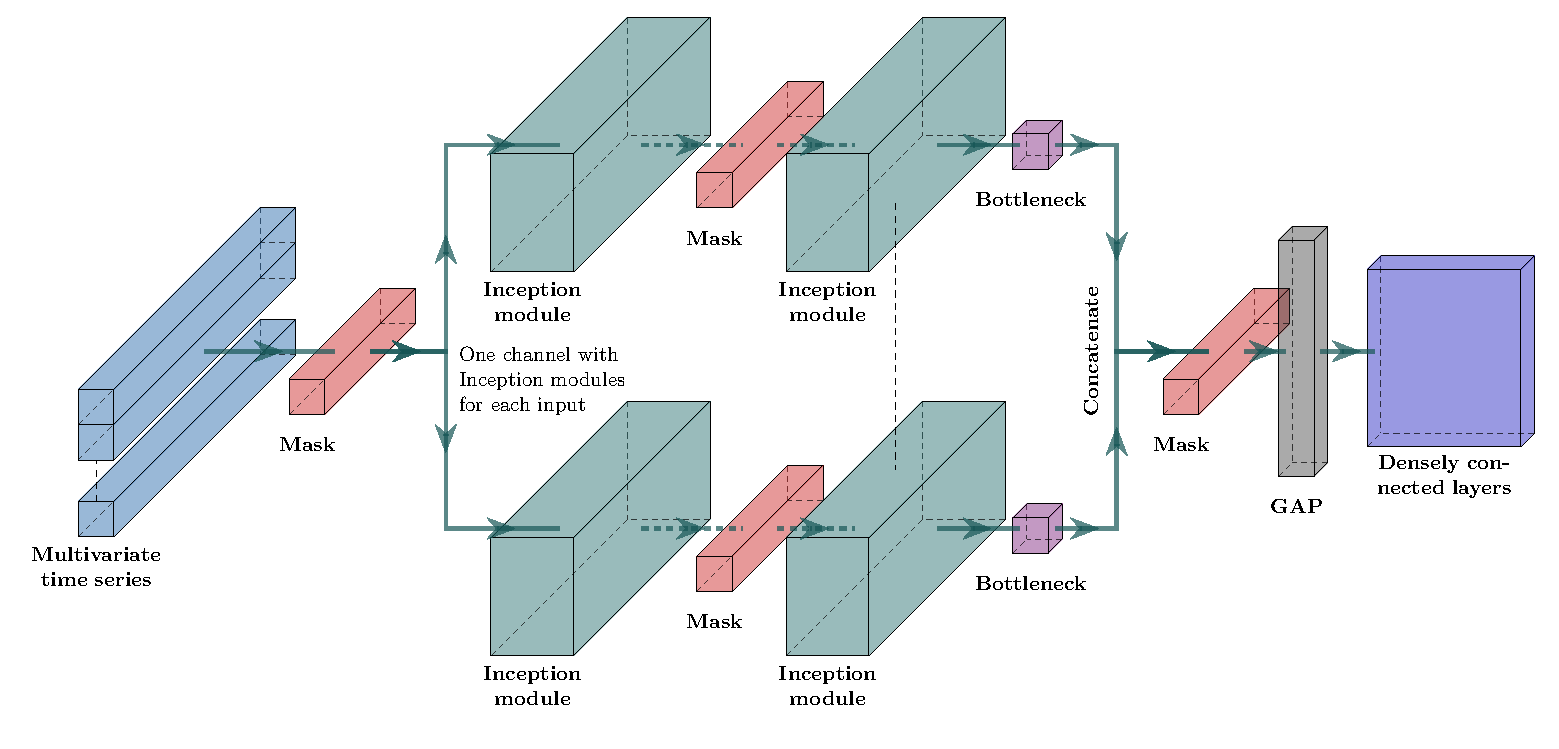
\includegraphics[width=\textwidth]{files/figs/met/x-inception-w-masks.pdf}
  \caption{The X-InceptionTime architecture developed in this work.}
  \label{fig:x-inception}
\end{figure}

The \gls{grad-cam} method is slightly modified and simplified for this model compared to what is presented in Section \ref{sec:grad-cam}, mainly due to the one dimensional data. Consider the final feature map $A$ consisting of the concatenated feature maps from the separate input channels. As mentioned above $A \in \mathbb{R}^{T \times F}$ and the aim is to find importance values for each time step in each input. With the same notations as in \eqref{eq:grad-cam}, i.e. $A_i^k$ corresponds to the activation of input $k$ at time step $i$, the \gls{grad-cam}, $M_c^k$, for class $c$ and input $k$ can be calculated as follows

\begin{align}
    \begin{split}
        w_k^c &= \frac{1}{T}\sum_{i=1}^T \frac{\partial y_c}{\partial A_i^k} \\
        M_c^k &= w_k^c A^k.
    \end{split}
    \label{eq:grad-cam-x}
\end{align}

 Compared to \eqref{eq:grad-cam} the $ReLU$ activation has been removed. This means that the importance values also contain information about which features suggesting this sample belongs to another class than $c$.

 Along with the effect of the time steps it is also possible, thanks to the \gls{gap} layer, to get a measure of the importance of each input. The importance value, $\alpha_k^c$, for input $k$ describes how much effect this input has on the classification decision. It is given by applying the \gls{grad-cam} method to the output of the \gls{gap} layer, $B$. From the feature map, $A$, this importance weight is calculated according to

 \begin{align}
   \begin{split}
      B^k &= \frac{1}{T}\sum_{i=1}^T A_i^k \\
      w_k^c &= \frac{\partial y_c}{\partial B^k} \\
      \alpha_k^c &= w_k^c B^k.
   \end{split}
 \end{align}

This was exploited to chose input features by iteratively training models, evaluating \eqref{eq:feat-select}, and removing the features corresponding to the lowest $W_k$ until the performance of the model drops significantly. This method has its drawback, the most notable that being that input features suitable for this architecture will be found. This model does not consider interaction between different features directly, hence features important through such interactions will probably not be deemed important by this method.

\begin{equation}
    W_k = \text{mean\_folds}\Big( \text{normalize}(\sum_{i=1}^N |w_{ik}^{c_i}|) \Big),
    \label{eq:feat-select}
\end{equation}
\begin{conditions}
  \text{mean\_folds}(z)   & = & average of $z$ over all folds \\
  \text{normalize}(z)     & = & $\frac{z}{\lVert z \rVert_2}$ \\
  c_i                     & = & argmax($\hat{y}_i$), i.e. the predicted class
\end{conditions}

\subsubsection{Ensembles}
The ensembles used consists of multiple models whose outputs are linearly combined to form the ensemble output. As discussed above this allows the ensemble to benefit from models optimized to perform well according to different metrics. In Section \ref{sec:met-training} we will present how $k$-fold cross-validation was used for training and validation. This was also used for design of the ensembles.

The idea with the ensemble was to combine models performing across all classes with models with high precision for the individual classes. The models with good overall performance was in general using the \gls{coral} activation and loss. The other models were trained with the confusion entropy loss with a target confusion matrix aiming at achieving high precision for one class and ignoring the other predictions. Examples of matrices used to find high precision models are shown in \eqref{eq:confusion-target}. A higher value can be seen as a reward for predictions turning up at that position in the confusion matrix. Eq. \eqref{eq:target-0} is used for class 0 and the ones in the lower right corner in this example means that correct prediction of a 1 will give the same reward as incorrectly predicting it as a 2.
The idea behind the lower reward for correct prediction of 0 together with the small rewards for predicting it as a 1 or 2 is to classify uncertain examples as 1s or 2s. The idea for class 2, in \eqref{eq:target-2} is the same, but opposite. As the underlying scoring scale is ordinal the same approach was not suitable for class 1. Instead a target matrix like \eqref{eq:target-1} was used. An alternative way of achieving high precision models was to tune the weight parameters $\lambda$ in the \gls{coral} loss, \eqref{eq:coral-loss}, to emphasize one of the rank predictions over the other.

% \begin{equation}
%     U = \begin{bmatrix}
%       0.6 & 0.05 & 0.05 \\
%       0 & 1 & 1\\
%       0 & 1 & 1
%     \end{bmatrix}
%     % \label{eq:confusion-target}
% \end{equation}


\noindent\begin{subequations}
\begin{minipage}{.33\textwidth}
  \begin{align}
  \label{eq:target-0}
  \begin{bmatrix}
    0.6 & 0.05 & 0.05 \\
    0 & 1 & 1\\
    0 & 1 & 1
  \end{bmatrix}
\end{align}
\end{minipage}%
\begin{minipage}{.33\textwidth}
  \begin{align}
  \label{eq:target-1}
  \begin{bmatrix}
    1 & 0 & 0 \\
    0.3 & 0.5 & 0.3\\
    0 & 0 & 1
  \end{bmatrix}
\end{align}
\end{minipage}%
\begin{minipage}{.33\textwidth}
  \begin{align}
  \label{eq:target-2}
  \begin{bmatrix}
    1 & 1 & 0 \\
    1 & 1 & 0 \\
    0.1 & 0.1 & 0.4
  \end{bmatrix}
\end{align}
\end{minipage}
\label{eq:confusion-target}
\end{subequations}

For the ensemble output the outputs of the individual models were combined as a weighted sum, according to

\begin{align}
    \begin{split}
      \mybar[0.7][1pt]{y}^{(c)} &= \sum_{i=1}^E w_i^{(c)} \widehat{y}_i^{(c)}, \\
      1 &= \sum_{i=1}^E w_i^{(c)}, \quad \forall c,
    \end{split}
\end{align}
\begin{conditions}
  E                   & = & number of ensembles \\
  \mybar[0.7][1pt]{y} & = & ensemble output \\
  \widehat{y}_i       & = & output if the $i$-th model.
\end{conditions}

The weights were determined based on the performance during the cross-validation and the weights for the precision models were set to zero for the classes it was not trained for.

The ensembles used are presented in Table \ref{tab:ensemble-models}. The suffixes -coral and -conf-X indicates \gls{coral} classifiers and models trained with the confusion entropy loss respectively. The X tells which was the high precision class. This is also used to indicate \gls{coral} models trained to achieve high precision. The depth, filter length, and number of filters for all X-InceptionTime models were 1, 31, and 32. The corresponding parameters for the InceptionTime models were 2, 31, and 128. Detailed model descriptions can be found in Appendix \ref{APPENDIX NGNSTANS} along with its training and ensemble weights.

\begin{table}
 \centering
 \caption{Models forming the ensembles. * indicates data length normalized to 100 samples. No star means that original sample frequency (25Hz) was kept and .}
 \label{tab:ensemble-models}
 % \footnotesize
 % {\renewcommand{\arraystretch}{1.2}
 % {\tabulinesep=0.8mm
 \small
 \begin{tabu}[t]{l:l:l:l}
   \textbf{Trunk} & \textbf{Pelvis} & \textbf{Femoral Valgus} & \textbf{\gls{kmfp}} \\
   \hline \hline

   InceptionTime-coral*     & & InceptionTime-coral*    & \\
   InceptionTime-coral      & & X-InceptionTime-coral*  & \\
   X-InceptionTime-conf-0*  & & X-InceptionTime-conf-0* & \\
   InceptionTime-conf-1*    & & X-InceptionTime-conf-1  & \\
   X-InceptionTime-coral-2  & & X-InceptionTime-conf-2* &
 \end{tabu}
\end{table}

% The models we used in the ensembles can be divided into three categories, i) models with good overall performance, ii) models with high precision for a specific class, and iii) models with high recall for a specific class. We found regular cross entropy and \gls{coral} models be suitable for the first category. This category forms the base of the ensemble and also works as a baseline to compare against. Unless the ensemble performs better than these individual models it does not serve any purpose. The second category, models with high precision,


% coral osv. custom losses osv?

\subsection{Training} \label{sec:met-training}
We used 10-fold cross-validation on the training set for the development of the models and ensembles. Like the test set, the folds were created such that no repetitions from the same subject were in both the test and validation set. For all models a batch size of 32, a learning rate of $5 \times 10^{-3}$, and early stopping was used. The learning rate was also reduced by a factor of 0.85 every 50th epoch. The training was performed on Nvidia Tesla T4 and V100 \glspl{gpu}.

% \subsection{Choice of input features}

\subsection{Combined score}
The eventual score in the method proposed by Nae et al. \cite{Nae2020b} is the combined assessments of all the repetitions. This score is formed as the median of the repetition scores. We propose to do this by averaging the ensemble outputs instead and chose the class with highest average probability over all repetitions. This means that a repetition classified with some uncertainty will affect the combined score less than a certain one. By evaluating the distributions for the ensemble outputs (Appendix \ref{LOL}) it is also possible to introduce thresholds for both the combined score and the repetition score. For the repetition predictions suitable thresholds and actions were found to be to set the probability to 0 if below 0.15. We also one hot encoded the prediction if the probability for one class was above 0.85.
